% setup
\nonstopmode
\documentclass[11pt]{article}
\usepackage{abstract}
\usepackage{amsmath}
\usepackage{array}
\usepackage[hypcap]{caption}
\usepackage[font=small,width=\textwidth]{caption}
\usepackage{color}
\usepackage{enumerate}
\usepackage{enumitem}
\usepackage{fullpage}
\usepackage{graphicx}
\usepackage{hyperref}
\usepackage{listings}
\usepackage{longtable}
\usepackage{microtype}
\usepackage{url}

% biblatex
\usepackage[style=ieee,backend=bibtex]{biblatex}
\addbibresource{voip}

% don't highlight links
\hypersetup{hidelinks}

% lists
\setlist[enumerate]{itemsep=-0.25em}
\setlist[itemize]{itemsep=-0.25em}

% general commands
\newcommand{\todo}[1]{\textcolor{red}{\textbf{TODO:} \emph{#1}}}
\newcommand{\term}[1]{\textit{#1}}
\newcommand{\bterm}[1]{\textbf{\textit{#1}}}
\newcommand{\code}[1]{\texttt{#1}}
\newcommand{\super}[1]{\textsuperscript{#1}}
\newcommand{\sub}[1]{\textsubscript{#1}}

% title
\title{VoIP: The present and future of voice communications}
\date{}
\author{
	\begin{tabular}{ c c c }
	Curtis Free \\
	\small \href{mailto:curtis.free@gatech.edu}{\nolinkurl{curtis.free@gatech.edu}} &
	\end{tabular}
}

\begin{document}
\maketitle

\section{Introduction}

What is \term{VoIP}? Most simply, Voice over Internet Protocol, or VoIP, is a
way of sending voice data over the Internet (or, in fact, any network that
supports IP). Just as a large portion of paper mail has been replaced with
electronic mail, voice calls are increasingly being transmitted around the world
via the Internet.

This paper will begin by describing how conventional telephony works. We will
then consider why we might want to improve upon conventional telephony with
something like VoIP and continue on to understand how VoIP actually works, both
in general and in specific systems with which you might be familiar. We will
then discuss the future of VoIP, paying particular attention to the emerging
VoLTE technology, and conclude with some observations about the role VoIP will
play going forward.

\section{Conventional telephony}

In order to understand how VoIP improves upon existing technologies, and why
even major telephony companies are adopting VoIP, it is instructive to examine
how conventional telephony works.

\subsection{PSTN}

Traditional telephone calls make use of the Public Switched Telephone Network
(PSTN) \cite{howstuffworks}. The PSTN is the regulated network of physical,
copper wires connecting most homes and businesses, coupled with the
carrier-owned backbone to this infrastructure. When a homeowner purchases
telephone service (or some other services such as DSL) from a telephony company
such as AT\&T or Windstream, that company manages the data sent over the
customer's wires. \cite{about}

Since its creation, PSTN has evolved from an analog-only network to one whose
backbone is mostly digital. Though originally developed for telephone service
specifically, its ubiquitous nature and its ability to transmit data among
locations across the globe has led to the development of other technologies,
including Internet access, piggy-backing off the PSTN. \cite{linfo}

\subsection{Voice encoding}

A telephone connected to the PSTN must translate sound waves into a data format
to be sent into the network; the algorithm used to perform this transformation
is called the \term{codec}. The standard codec used in PSTN is G.711, a digital
format in which sound snapshots called \term{samples} are captured at specific
intervals, encoded, and transmitted, uncompressed, through the PSTN to their
final destination. \cite{coding,vostron}

\subsection{Circuit switching}

The most notable aspect of conventional phone service is that connectivity
between speakers (or endpoints, in the case of something like DSL) is
circuit-switched. This means that while the speakers are both ``on the line,''
there is a single path through the PSTN over which all traffic between the two
parties will pass.  As one party speaks, the voice data transmission follows
that unitary path to the other party; and speech in the reverse direction
travels over the same set of physical links. \cite{privateline} Figure
\ref{fig:conventional} depicts a circuit-switched telephone connection.

\begin{figure}
	\centering
	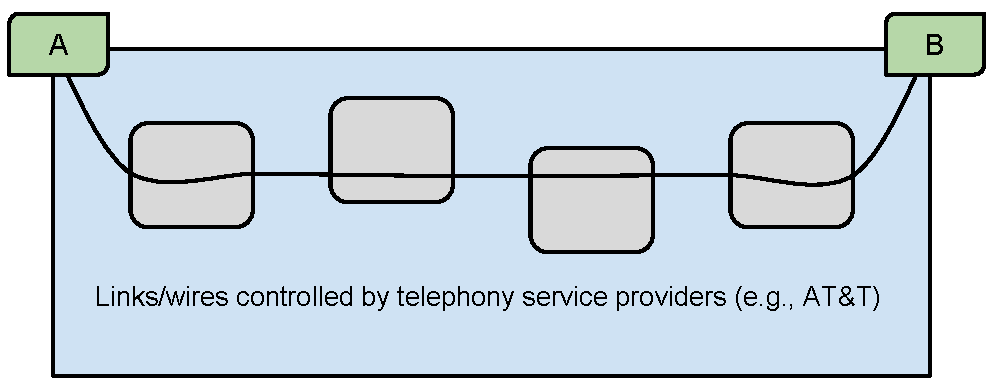
\includegraphics[width=\textwidth]{circuit_switched}
	\caption{
		In a conventional telephone network, such as the PSTN, a path is established
		between callers $A$ and $B$. All voice data exchanged between the two, for
		the duration of the call, flows along the same network path.
	}
	\label{fig:conventional}
\end{figure}

The PSTN supports simultaneous communication through the use of \term{time
division multiplexing} (TDM); in other words, an underlying protocol determines
when the link will be used by each party that has been allocated a share of the
link. The path through the PSTN from a caller to a callee will pass along
multiple physical links, and for each physical link, the connection is allocated
a particular \term{circuit} determining when that connection will send data
across the link. \cite{pstn_ppt}

\section{Why VoIP?}

\subsection{Problems with PSTN}

The PSTN is a complicated network built and maintained for a very specific
purpose: to carry voice calls (though it has expanded to provide some other
services). This combination means that maintenance of the network requires very
specialized equipment and parts -- making ongoing maintenance very expensive.
Furthermore, it is difficult to make improvements in the underlying
communication mechanisms and protocols used on the PSTN because doing so would
require updated support in the backbone itself.  \cite{privateline}

So much so, in fact, that plans are currently underway to replace the PSTN with
a VoIP telephony backbone; AT\&T intends for its own transition to be complete
by 2020 \cite{networkworld,ars}. As we'll see later, VoIP will soon become the
standard mode of operation for mobile telephony, as well.

\subsection{Using the Internet}

The Internet powers an increasing number of devices and services; it provides a
rich and yet generic infrastructure with global reach -- allowing data to be
transmitted quickly from one location to another. With the prevalence of the
Internet, this infrastructure is only going to grow.

Due to its prevalence and its ability to transmit both a large amount of data
and any type of data that can be encoded digitally, the Internet lends itself to
the problem of \emph{globally-available} voice communications. In contrast with
PSTN, devices and equipment for use with the Internet are very cost effective
\cite{privateline}.  In addition to reducing the network maintenance costs, this
reduces the cost barrier to entry in the telephony market, allowing new
companies to provide products with ``unique features'' and fostering innovation
in an area that has largely become stagnant \cite{privateline}. Existing
services like Google Hangouts or Apple's iMessage blur the lines between modes
of communication -- combining Internet-based messaging with SMS (text) messages;
transmission of voice over Internet channels can allow similar bundling of rich
Internet-based services with communication methods typically served over PSTN
channels \cite{3gpp,privateline}. 

With the Internet, most transmission logic -- in particular, higher-level
transmission logic -- resides at the edges of the network. That is, the backbone
itself operates only at low levels, primarily performing low-level routing and
filtering. This characteristic means that the Internet -- and thus VoIP -- can
foster rapid innovation. End devices can be upgraded and improved at a rapid
pace without requiring changes to the core network infrastructure, which simply
routes data from one location to another. In this way, the flexibility of an
Internet-like architecture means that VoIP solutions can be updated and improved
upon easily.  This is not something than can be said about the PSTN due to its
specialized infrastructure. \cite{privateline}.

Another interesting feature available with VoIP but not directly possible using
PSTN is connection encryption. Because VoIP devices may communicate in any way
they wish, as long as the devices on each end of the connection understand the
same protocols and techniques, communication between them can optionally be
encrypted -- as is the case with communication between customers of the Skype
service. \cite{skype_encryption}

\section{How VoIP works}

\term{VoIP} stands for \term{Voice over Internet Protocol}. Internet Protocol
(IP) is a mechanism used to send small pieces of data, called ``packets,''
across the Internet from source to destination. VoIP is a generic term used to
refer to any system whose purpose is to transmit voice data between two parties.
\cite{goode}

\begin{figure}
	\centering
	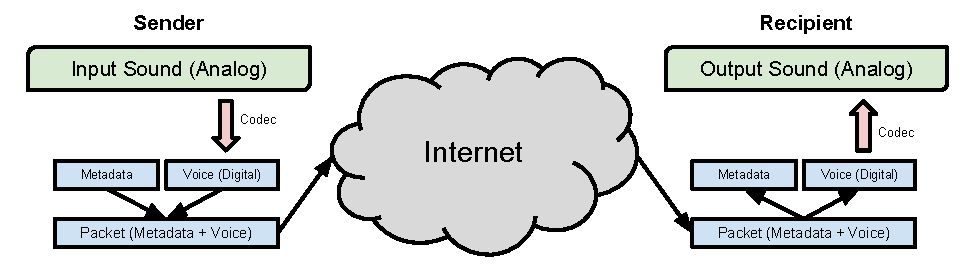
\includegraphics[width=\textwidth]{voip_diagram}
	\caption{
		How VoIP transmits sound data from a caller to a callee.
	}
	\label{fig:voip_diagram}
\end{figure}

Figure \ref{fig:voip_diagram} depicts VoIP at a high level. Voice data at the
microphone on the sender is captured in samples, encoded as bits using a
configurable codec, and sent to the recipient. This is much true of both PSTN
and VoIP systems; however, \emph{what} is sent is \emph{how} it is sent differs.

With VoIP, the encoded voice data is bundled with metadata about the receiving
party and sent out a network link into the Internet, where it will be routed in
much the same manner as email messages and Web pages.

The \term{packet-switched} nature of the Internet, as well as the important
tradeoffs involved in this technology, highlight the differences between VoIP
and conventional PSTN telephony.

\subsection{Packet switching}

Whereas voice data via conventional channels is streamed over a single path
between source and destination, VoIP -- and the Internet as a whole -- work in a
fundamentally different way.

Devices using Internet Protocol (the \term{IP} in \term{VoIP}) transmit
information in separate, small packages called \term{packets}. Each packet
contains a \term{body} of data to be transmitted (e.g., the encoded voice data)
and a \term{header} providing, at a minimum, the IP address to which the voice
data should be sent. Depending on the solution, this address will be that of the
callee or that of a VoIP support server.

Packets are routed through devices across a wide variety of networks between
their source and destination. A number of protocols are used throughout the
network to determine the most appropriate way to route packets toward their
respective destinations.

\begin{figure}
	\centering
	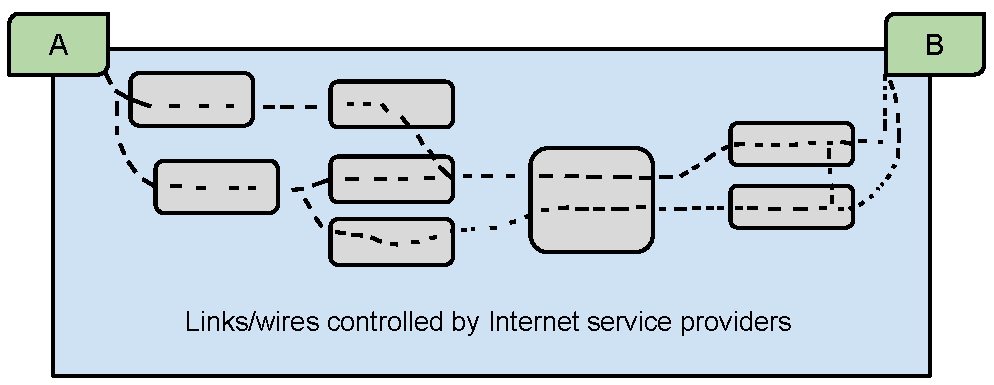
\includegraphics[width=\textwidth]{packet_switched}
	\caption{
		A \term{packet-switched} data exchange between $A$ and $B$. Voice data is
		sent between the parties in \term{packets}.
	}
	\label{fig:packet_switched}
\end{figure}

Often, a number of packets between a particular source and destination
\emph{will} follow the same path; however, the manner in which the protocol
works -- constantly attempting to determine the best path and adjusting
appropriately, possibly even sending data via multiple paths -- is fundamentally
different from circuit-switched networks such as the PSTN, which always send
data over the same dedicated (but possibly-shared) channel. \cite{packets}
Figure \ref{fig:packet_switched} depicts data traversing a packet-switched
network.

With VoIP, as with the PSTN, physical network links must be shared. This is a
problem inherent to a packet-switched network, and a number of strategies have
been devised for dividing link access -- including TDA, as with the PSTN. A full
review of these techniques is outside the scope of this paper.

\subsection{Delivery}
\label{sec:voipdelivery}

Many applications of the Internet -- such as Hypertext Transfer Protocol (HTTP),
which powers the Web -- require that the recipent have \emph{all} of the data
provided by the sender. For example, a Web page cannot necessarily be displayed
if portions of its data are absent. To accommodate this, a protocol called the
Transmission Control Protocol (TCP) is used to ensure that the sender re-sends
data that is not received by the recipient. The overhead involved in ensuring
this \term{reliable delivery} can be significant, as it requires that the two
parties send a wealth of state information to one another. With voice data, it
is more important that the recipient receive \emph{as much data as possible in a
timely fashion}. That is, having most of the voice data produced by the sender
is sufficient to understand the sender's speech, and any efforts to ensure that
all data is received simply result in a delay on the recipient side, which is
more disruptive to communication than small portions of missing data.
\cite{goode}

In contrast, most VoIP communication makes use of the alternative User Datagram
Protocol (UDP), which sends packets without retransmission; Real-time
Transmission Protocol (RTP) is a layer atop UDP which is designed to facilitate
streams of time-sensitive information such as voice data. \cite{goode,rtp_voip}. 

RTP is often (though not always \cite{goode}) used alongside Real-time
Transmission Control Protocol (RTCP), which in the case of VoIP is used to send
non-voice informational messages between hosts. This includes information used
when establishing a connection and information about the quality of the
connection and ongoing connection statistics during the length of the call
\cite{voipinfo_rtp,rtp_voip}.

Realizing that some data might be lost during transmission, a recipient VoIP
device can actively modify the perceived sound to reduce disruption when this
occurs. This technique is called \term{packet loss concealment}. When packets
are not available to provide the appropriate sounds for a particular point in
time, the device can simply remain silent, hold out tones that have been
received, or even attempt to reproduce a reasonable next sound. \cite{coding}

Thus, VoIP systems are able to use choice protocols and techniques to reduce
degradation of sound quality that could otherwise result from using the Internet
as a transport mechanism.

\subsection{Encoding and bandwidth}

Another important problem in the design of a VoIP system is how the available
bandwidth can be used efficiently. In the case of PSTN, senders and recipients
have a dedicated 64 kbps of communication bandwidth \cite{privateline} -- but
over the Internet, where voice data must compete with other types of data such
as image and video downloads, it is important to conserve bandwidth while still
providing adequate voice quality.

In order for voice data to be transmitted across the Internet, it must be
translated from analog sound waves into binary data -- \term{bits}. Like PSTN
communications, VoIP systems must use a codec, which determines how voice data
is translated into binary data and -- on the receiving end -- how the reverse
transformation is performed \cite{goode}. As long as both the sender and the
recipient understand the same codec, they can communicate using data exchanged
via the Internet. Different codecs have different characteristics. In
particular, the codec determines the amount of data that must be transmitted to
convey speech and the overall quality of the sound reproduction: bandwidth
savings can be achieved by reducing data usage, but at the cost of quality.
\cite{goode}

Note that it is possible for a VoIP implementation to use the same codec as the
PSTN: G.711. In fact, VoIP provider Vostron does exactly that. According to
Vostron, this provides good quality -- but at a higher bandwidth cost than other
codecs that make use of compression. \cite{vostron}

To compress voice data means to process it using a special algorithm so that the
same data -- or roughly the same data -- can be represented using fewer bits.
Unfortunately, the cost of compression is some delay in communication.
\cite{goode} Because voice data is transmitted using a large number of packets,
each containing a small amount of information, \term{header compression} is used
in some VoIP systems to reduce the number of bits of packet-level metadata that
must be transmitted; otherwise, the size of this metadata contributes
significantly to the size of a packet \cite{hsdpa}.

Interestingly, there are also techniques to reduce the amount of data exchanged
when one or both parties in a call are silent. Most simply, when a VoIP device
detects that the speaker has ceased talking, such that only background noise is
heard, a minimal amount of data can be transmitted such that the receiving end
hears only silence. A more advanced alternative is to send a small amount of
data allowing the recipient to reconstruct sound that is \emph{similar} to the
actual background noise on the sending side -- which requires fewer bits than
transmitting the entirety of the actual background noise and yet is less jarring
to the recipient hearing a jump between stark silence and speech. \cite{goode}

\subsection{VoIP and PSTN interconnectivity}

Until VoIP backbones have entirely replaced the PSTN, many VoIP callers must be
able to communicate with PSTN recipients and vice-versa.

In order to support interoperability between VoIP systems and the PSTN, voice
providers use ``gateway'' devices which can translate from one data format to
another \cite{goode}. When a VoIP caller speaks with a PSTN party, or when data
is routed across the two systems for another reason, the connection between the
two parties is of a mixed nature: at some points along the path, a channel is
established to provide circuit-switched connectivity; but packet switching is
used elsewhere in the path.

Specific protocols have been developed to facilitate efficient communication
between these two systems. Telephony Routing over IP (TRIP) is one such
protocol: TRIP can be used to determine how particular calls can be routed
across VoIP and PSTN to get to the appropriate destination \cite{goode,trip}.
However, a different protocol -- ENUM -- is used in practice. ENUM uses DNS to
allow a caller using one technology to locate the underlying address necessary
to reach another caller. \cite{goode} Given a particular phone number that has
been dialed, information returned by the ENUM record(s) tells the caller how the
party being called should be reached. \cite{voipinfo_enum}

For example, suppose that Bob uses his AT\&T cell phone to call Alice, who uses
a VoIP phone from Vonage. After Bob dials Alice's number, AT\&T will realize
that Alice's number is not serviced directly by PSTN. It can then look up her
number in an ENUM directory to determine the Internet location that should be
contacted in order to send voice data to Alice.

\section{Example implementations}

There are many different implementations of VoIP. For illustrative purposes and
to demonstrate the variety of existing VoIP systems, we will survey three
common examples: Vonage, Skype, and Cisco's IP phones.

It is important to note that VoIP service can be dividied into two
subcategories: those that are designed specifically to interface with
circuit-switched networks and those that are designed primarily to communicate
with other VoIP clients. In the former case, as with Vonage, end users are each
assigned a ``globally'' addressable telephone number that can be reached from
any telephone, whether VoIP or circuit-switched; in such cases, there must be
appropriate gateways bridging the packet-switched and circuit-switched networks.
But in the latter case, as in Skype and a number of other Internet-enabled chat
applications, clients can communicate by identifying one another using
service-specific identifiers outside the typical telephone number system. It is
possible in some of these systems to make bridged calls to phones reachable via
PSTN.

\subsection{Vonage}

Vonage is a popular VoIP service provider supporting calls via both home
telephones and mobile phones; in particular, we will discuss how Vonage works in
relation to home phones.

Vonage provides subscribers with a conversion device to be installed in the home
known as an \term{analog telephone adapter}, or \term{ATA}
\cite{vonage,howstuffworks}. This device acts as the translator between the
phone's analog output and the digital Internet, allows a Vonage customer to use
a conventional in-home telephone with Vonage's VoIP service.

The Vonage ATA routes both control and data packets to Vonage servers, from
which it can be routed further to a PSTN gateway or to another Vonage server.

In order to complete calls, Vonage makes use of the Session Initiation
Protocol (SIP) \cite{dslreports,skype_vs_vonage,ipwatchdog}. When a
user places a phone call via Vonage, the ATA begins by sending appropriate SIP
messages to the Vonage servers. SIP messages indicate such things as (a) who is
making the call, (b) who is being called, and (c) what services the sender
supports. \cite{sip} SIP relies on RTP and RTCP, discussed in
Section \ref{sec:voipdelivery}, for underlying communication between devices.

When making a call via a VoIP provider like Vonage, SIP is used to perform the
initial \term{handshake} between caller and callee. SIP messages allow a caller
to inform the callee that a call is incoming and allow the callee to respond.
After the handshake has taken place, the caller and callee are ready to begin
voice communication. \cite{rtp_voip}

\subsection{Skype}

Skype differs from services like Vonage in specific ways. In particular, Skype
is designed to be run from a computer or smartphone rather than from
conventional analog-output phones. Skype users are not assigned a particular
telephone number from the PSTN.  Rather, Skype assigns each user a
Skype-specific identifier that can be used to make calls. Skype users can
choose, however, to make calls to PSTN endpoints, at which point a gateway is
used to enable such communication.  \cite{skype_pstn,skype_gateways}

A notable feature of Skype is that it is designed as a peer-to-peer (P2P)
system. As such, when a call is made between Skype users, the caller finds the
callee by communicating with its peers -- other hosts running Skype -- rather
than a central Skype server. \cite{skype}

Unfortunately, as a closed-source system, the details of Skype's implementation
are known only from black-box observation, as in \cite{skype}. In some cases,
Skype uses proprietary techniques rather than more established protocols such as
SIP, RTP, and RTCP.

\subsection{Cisco IP phones}

Cisco IP phones are designed for use in a corporate environment. Whereas in-home
VoIP devices such as those provided by Vonage communicate directly with the
provider's own servers, Cisco phones are designed to communicate with an
in-house VoIP backbone that is hosted and manged by the corporation itself. In
fact, VoIP is only used \emph{within} the implementing organization: the
internal backbone interfaces with the PSTN so that the organization's phones are
entirely compatible with conventional phones. \cite{cisco_design}

For a large organization with many telephone endpoints, using IP phones -- even
if only internally -- can simplify the IT infrastructure since it only need
manage a wide-area network (WAN) within the company/building. This
infrastructure is likely already in place to support intranet and Internet
access. Additionally, within the organization, Cisco-to-Cisco calling can take
advantage of advanced features like video calling \cite{tmcnet}.

\section{Coming soon: VoLTE}

Though there are no wires directly connecting wireless handsets and cell towers,
at its heart even cellular telephones communicate with each other and with
conventional phone terminals using circuit-switched connections. While this mode
of operation is straightforward for simple devices, data-enabled smartphones
(and tablets) make use of wireless signals to connect to the Internet, and for
the same reasons as above, transmitting voice signal over the packet-switched
Internet can be a cost-effective strategy.

\subsection{Voice over LTE}

Older cellular data technologies -- those known as \term{2G} and \term{3G} --
support exchange of voice information between the handset and a tower via the
same channel as the data; that is, voice can be transmitted over 2G/3G. However,
recently \term{4G LTE} has become a popular form of data communication due to
its significantly faster data transfer speeds. \cite{volte_book}

In terms of voice communication, however, LTE is is some ways \emph{forcing}
carriers to move toward VoIP. This is because unlike 2G and 3G, LTE is designed
to handle only IP-based traffic. \cite{3gpp}

As an interim solution, carriers currently make use of \term{circuit-switched
fallback} (CSFB): when a device using LTE wishes to place a voice call, the
device uses its 2G/3G radio to place the call. \cite{volte_book} Ideally,
however, with an increasing number of carriers offering LTE data connectivity,
that channel could be used to transmit voice calls, freeing carriers to phase
out old radios and focus their network efforts on newer technologies such as
LTE.

The \term{OneVoice} initiative, begun in 2009, is a cross-carrier effort to
develop and adopt a unified solution to provide VoIP via LTE -- known as
\term{Voice over LTE}, or \term{VoLTE}.  While carriers could engage in
stovepiped development of individual solutions, OneVoice lays out a plan by
which all carriers will implement VoLTE in the same way, easing compatibility
between networks. OneVoice champions the IP media subsystem (IMS), an IP-based
framework for providing media such as voice over the packet-switched IP layer.
OneVoice goes further, however, actually specifying both hardware and software
requirements that must be met so that customers will experience acceptable
performance when using VoLTE with any of the OneVoice participants.
\cite{volte_book}

An existing component of LTE systems, the \term{evolved packet core} (EPC) can
help provide VoLTE services: EPC can act as a gateway between the
LTE-transmitted IP packets and the remaining circuit-switched telephony networks.
\cite{volte_book}

Furthermore, a principle purpose of IMS and reason for its adoption in the
mobile telephony area is to provide a common API for voice services regardless
of the transport mechanism. If IMS were supported by all carriers and internet
service providers, then it would be possible for a mobile telephone to send VoIP
data over whatever internet connection is available -- whether that be VoLTE or
WiFi. \cite{f5}.

Despite having reached a consensus that IMS is the path forward, however,
existing carriers now face the internal burden of adapting their particular
technologies to work with VoLTE; that is, though the end goal is the same across
carriers, the paths used to get there must vary widely. \cite{theregister}

Even today, some cost-conscious subscribers make use of third-party VoIP
solutions, such as Skype or GrooveIP, to make calls via data connection. While
such solutions work to some extent, first-class VoLTE has the potential to
provide much better performance (and thus better call quality) than these
solutions because carriers will be motivated to provide first-rate QoS to ensure
that VoLTE packets receive priority over non-voice traffic. \cite{theregister}

\subsection{Current VoLTE status}

Testing in 2012 suggested that VoLTE could have a significant \emph{negative}
impact on battery life \cite{dlvoltestudy}. It is widely known that LTE radio
drains mobile device batteries; however, as LTE networks have seen increased
adoption in recent years, it is likely that newer devices designed for VoLTE
could see better results than those experienced in early testing.

Some wireless carriers are currently developing their VoLTE solutions. U.S.
carrier Verizon Wireless plans to make VoLTE available in 2014 \cite{vzwvolte}.

Even with initial VoLTE offerings in store in the near future, this technology
will not be viable as a complete alternative until LTE coverage is at least as
extensive as today's data coverage. In the case of Verizon's network technology,
calls made over VoLTE cannot be handed off to non-LTE channels, and so these
carrier-driven VoIP calls are still only usable in a limited (but growing) area.
\cite{dzvzwvolte}

\section{Continued challenges}

A challenge on the part of a traditional carrier moving to VoIP is that of
\emph{billing}. When data is simply sent into the Internet rather than across
the telecom-controlled PSTN links, how can a company determine how much a
customer should be charged for a particular call? In particular, traditional
calling charges are based on the duration of the call because during that time,
the user is allocated a portion of the network for circuit-switched
communication. This is no longer true with VoIP. \cite{theregister}

Another significant challenge is operation of the Emergency 911 system for
callers using VoIP. With PSTN, 911 responders can determine with certainty where
a particular call originated because telephone numbers are registered to
particular georgraphical addresses, allowing response to calls even when the
caller cannot identify the location. But with VoIP, call data emanates from a
particular IP address, and mapping an IP address to a specific geographic
location is not as certain a practice. \cite{howstuffworks} For the time being,
at least, some in-home VoIP services make use of the PSTN and can therefore
determine a caller's location in the case of an emergency \cite{us_cert}.

An often-cited drawback of VoIP is reduced reliability. Namely, the PSTN has a
reputation for providing reliable access, but Internet connections regularly
experience outages of varying severity. \cite{howstuffworks} As mission-critical
services such as telephony get pushed into the network, we can expect that new
strategies and technologies for increasing network reliability will appear. When
it does, this will have a positive impact on all services that make use of the
Internet.

An additional challenge is that of security. Though PSTN has seen attacks in the
past, its tightly-controlled network means that an attacker cannot easily
perform attacks such as man-in-the-middle. With Internet-powered services, we
must consider such attacks. How does a caller know that the person on the
receiving side is in fact the correct party? Alternatively, can attackers bring
down a company's telephone infrastructure by performing a distributed
denial-of-service attack on a particular port? As VoIP becomes more popular,
attention must be afforded to its security.

\section{Conclusion}

Transition from PSTN to VoIP is inevitable, and work to make this transition is
already underway. The simplicity of managing a single communications network is
attractive to the service providers managing today's telephony backbone.
Tech-savvy users will appreciate the ability to combine voice and other
services, and the ability to rely on wired and wireless LAN technologies rather
than phone-specific lines for voice communications in the home.

For the general public, the draw of VoIP is not as apparent. In the short term,
ideally, most users will not notice a difference when they begin using a
VoIP-powered backbone rather than the PSTN solution to which they are
accustomed. However, in the longer term, new and exciting voice services will be
built atop established VoIP back-ends.

VoIP is the next evolutionary step for voice communications. VoIP technology is
constantly being improved, and it will be for the foreseeable future.

\printbibliography

\end{document}

% vim: set inde= colorcolumn=81 textwidth=80 spell:

